\chapter[The Economics of Migration: The Migrant]{The Economics of Migration: The Migrant\raisebox{.3\baselineskip}{\normalsize\footnotemark}}
\footnotetext{Written by Kuangjie Ni, Edited by Xiaotian Tian}

\fancyhead[L]{ECON0024}
\fancyhead[C]{Ch.11 The Economics of Migration: The Migrant}
\fancyhead[R]{Kuangjie Ni}
\fancyfoot[L]{\hyperlink{tableofcontents}{Back to Table of Contents}}
\fancyfoot[R]{Kuangjie Ni}

\section{Introduction and Motivations}

    \subsection{Motivations}
    
        \begin{itemize}
            \item \emphb{Definition of Migration}: movement of individuals from one region to another
                \begin{itemize}
                    \item International migration: movement of individuals across international borders
                \end{itemize}
            \item \emphb{Causes for Migration}: 
                \begin{itemize}
                    \item Economic reasons (e.g. education, climate, amenities)
                    \item Persecution, displacement as a result of war or ethnic cleansing (very dominant in past decades)
                    \item Preference for the host country 
                \end{itemize}
            \item \emphb{Consequences of Migration}:
                \begin{itemize}
                    \item Host country: direct and immediate effects in economy and society along various dimensions (wages, fiscal effects, innovation, food, habits, etc.)
                    \item Source country: Immediate effects through withdrawing people (brain drain / brain gain), return and remittances. Also, return migration may bring back new skills and technology learned from the host country to the home country.
                \end{itemize}
            \item Economically motivated migration \empha{always generates a surplus}, but has distributional effects at the same time
                \begin{itemize}
                    \item The main beneficiaries of migration are the migrants themselves
                    \item Key questions: Who else gains in source and sending country, and who may lose?
                \end{itemize}
        \end{itemize}

    \subsection{Focus of Economic Research on Migration}
    
        \begin{itemize}
            \item Migrants:
                \begin{itemize}
                    \item Migration and re-migration decisions
                    \item Immigrant's performance in the receiving country
                    \item The selection of immigrants
                    \item The children of immigrants
                \end{itemize}
            \item Non-migrants in Host and Source Country:
                \begin{itemize}
                    \item Impact immigration may have on receiving country: wages, employment, prices, fiscal effects, innovations, crime, etc.
                    \item Impact emigration may have on the sending country: employment, wages, income, children's education, etc.
                    \item Analysis of remittances
                    \item Cultural consequences
                \end{itemize}
            \item The Interaction of Immigrants and Natives
                \begin{itemize}
                    \item Social cohesion, attitudes to immigration, social integration, political outcomes (e.g. voting outcomes)
                \end{itemize}
        \end{itemize}

    \subsection{Emprical Facts: Migration in the International Context}

        \subsubsection{Stock of Migrants}

            Immigration: used to be a phenomenon of the “New World,” but most developed Western nations today have large immigrant populations, and many Asian countries have large internal migration from rural areas to cities.

            \begin{itemize}
                \item World stock of international migrants (UN, Dept of Econ and Soc Affairs, 2019) :
                    \begin{itemize}
                         \item 1995: about 161 million people, 2.8 percent of the world population
                         \item 2019: almost 272 million, 3.5 percent of the world population
                    \end{itemize}
                \item Stock in Europe, Northern America, Australia/New Zealand and Japan :
                     \begin{itemize}
                         \item 1995: 92 million, 7.9 percent of the population
                         \item 2019: more than 150 million, 12 percent of the population
                    \end{itemize}
            \end{itemize}

        \subsubsection{Number of Migrants}
            
            \begin{figure}[H]
                        \centering
                        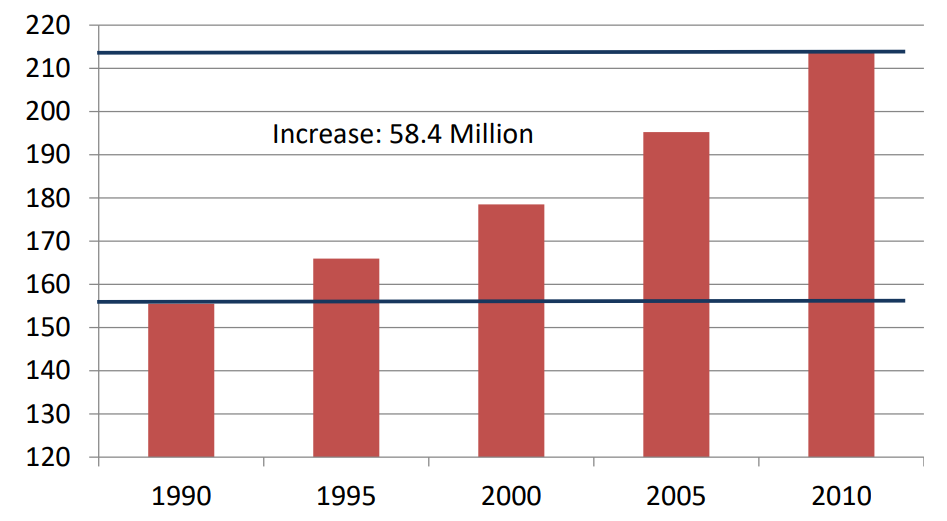
\includegraphics[width=4in]{images/ch11/1.png}
                        \caption{Estimated number of international migrants in millions}
                    \end{figure}
            For the whole world, there is a 58.4 million increase in the number of international migrants from 1990 to 2010, and this figure continues to increase.

        \subsubsection{Share of Migrants}

            \begin{figure}[H]
                \centering
                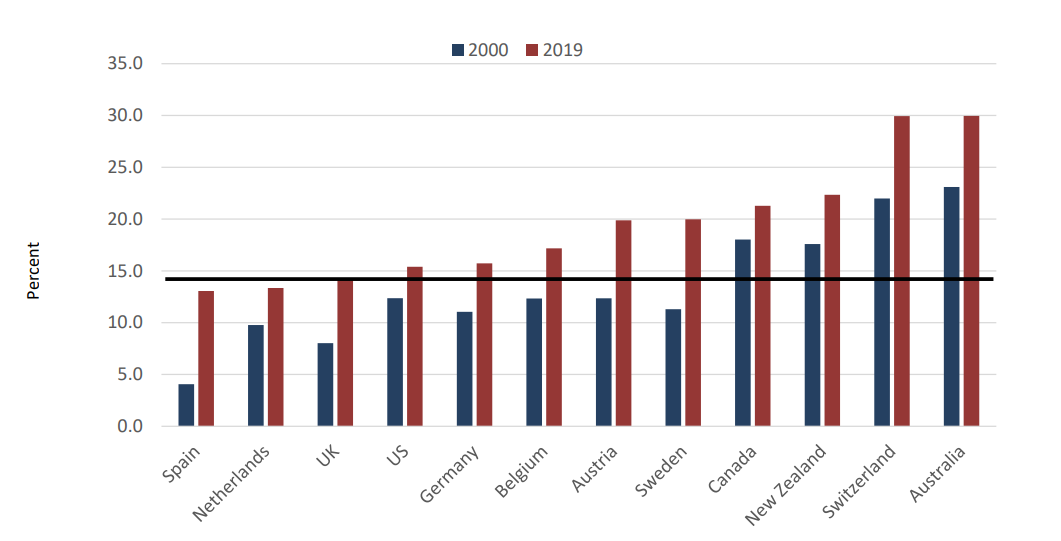
\includegraphics[width=4.5in]{images/ch11/2.png}
                \caption{Share of foreign-born population, selected countries}
            \end{figure}
            \begin{itemize}
                \item Blue bars indicate the shares of the foreign-born population in 2000, and red bars indicate the share of the foreign-born population in 2019. 
                \item The figure in Spain has tripled.
                \item In 2019, one in three people in Switzerland and Australia are foreign-born.
                \item The horizontal line is the 2019 average for the countries shown on the figure weighted by their total population.
            \end{itemize}

        \subsubsection{Education of Migrants}

            \begin{figure}[H]
                \centering
                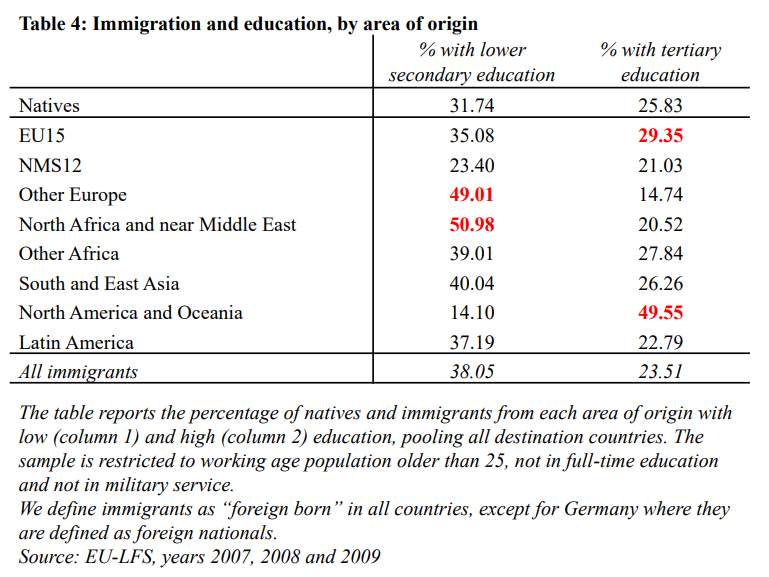
\includegraphics[width=4in]{images/ch11/6.png}
                \caption{Education of immigrants}
            \end{figure}
            \begin{itemize}
                 \item The table reports the percentage of natives and immigrants from each area of origin with low (column 1) and high (column 2) education, pooling all destination countries. The sample is restricted to the working-age population older than 25, not in full-time education and not in military service. We define immigrants as “foreign born” in all countries, except for Germany where they are defined as foreign nationals.
                 \item The share of immigrants with lower secondary education is high (around 50 percent) in Other Europe,  North Africa and near Middle East. The share of immigrants with tertiary education is high (around 50 percent) in North America and Oceania.
            \end{itemize}

    \subsection{Empirical Facts: Migration in the European context}

        \subsubsection{Brief History of 5 Waves of Migration to Europe}

            \begin{itemize}
                \item Europe experienced \emphb{five major migration waves} after WW2.
                \item 1945 - 1960: Migrations caused by the war. About 20 million people displaced, mainly Germans.
                \item Second migration movement: economically motivated, started in the early 1950's - 1973 (labour migrations).
                \item Third wave of migration after 1973: family immigration and reunification of former labour migrants, and asylum migration.
                \item Fourth big movement: East-West migration, initiated in the late 1980's by a liberalisation of Soviet policy and accelerated by the fall of the Berlin wall in 1989.
                \item Early 1990’s: Movements as consequence of independence and democratisation, of wars inflicted on many areas within and around Europe.
                \item 2000’s: Globalisation, EU enlargement, and labour market rigidities let to large immigration flows into, and across European countries.
                \item Question: Next decade? Immigration is likely to be increasingly fueled by war prosecution and inequality. Also, social media make people easier to get information about the host countries and then move.  Moreover, the large increase in population in Africa and, thus, the immigration imposes pressure on Europe and the US.
            \end{itemize}

        \subsubsection{Immigrants across Europe: Percentage and Origin}

            \begin{figure}[H]
                \centering
                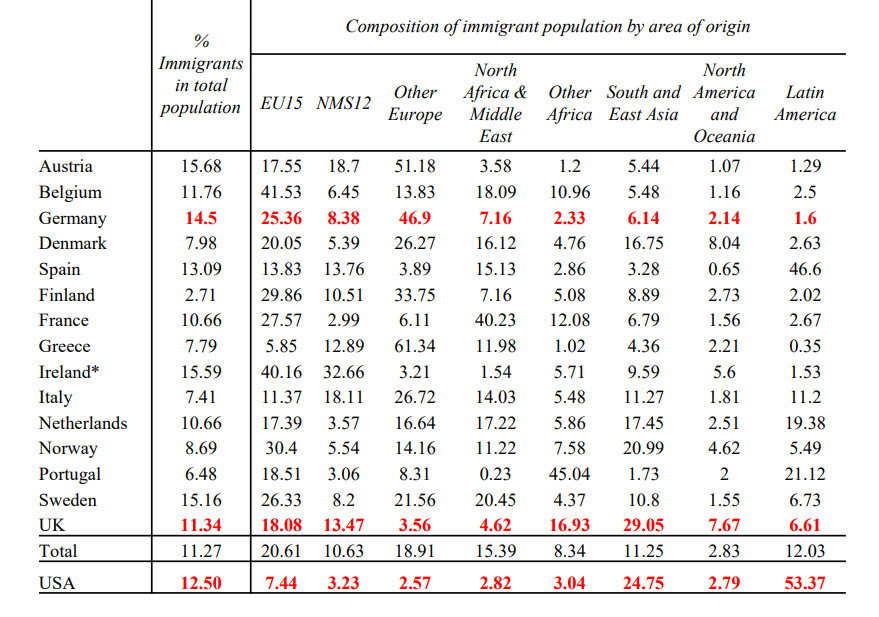
\includegraphics[width=4in]{images/ch11/3.png}
                \caption{Immigrants as a percentage of the total population, years 2007-2009}
            \end{figure}

            There is a large difference in immigrant shares across different countries, and the composition by area is different.

        \subsubsection{Education}

            \begin{figure}[H]
                \centering
                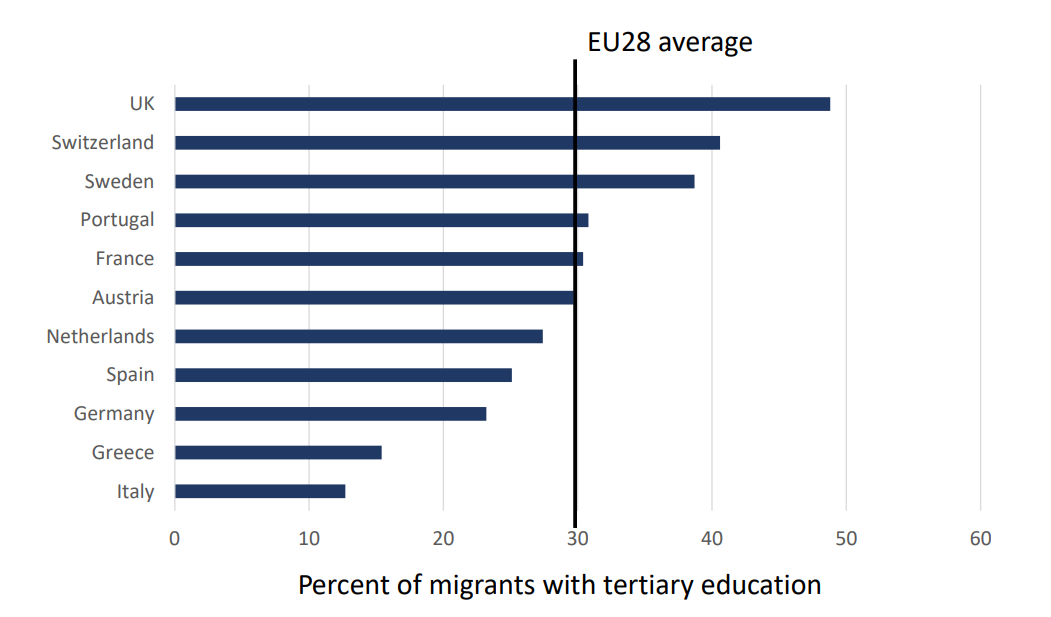
\includegraphics[width=4in]{images/ch11/4.png}
                \caption{Share of immigrants with tertiary education in selected EU countries, 2018}
            \end{figure}
            
            \begin{itemize}
                \item Immigration is not a homogeneous phenomenon across countries. It is different in terms of education and origins across countries. 
                \item On average in EU28, one in three immigrants has tertiary education.
                \item The UK attracts the best-educated immigrants. Germany has a relatively low proportion of immigrants with tertiary education.
            \end{itemize}

        \subsubsection{Composition of Foreign-Born Population}

            \begin{figure}[H]
                \centering
                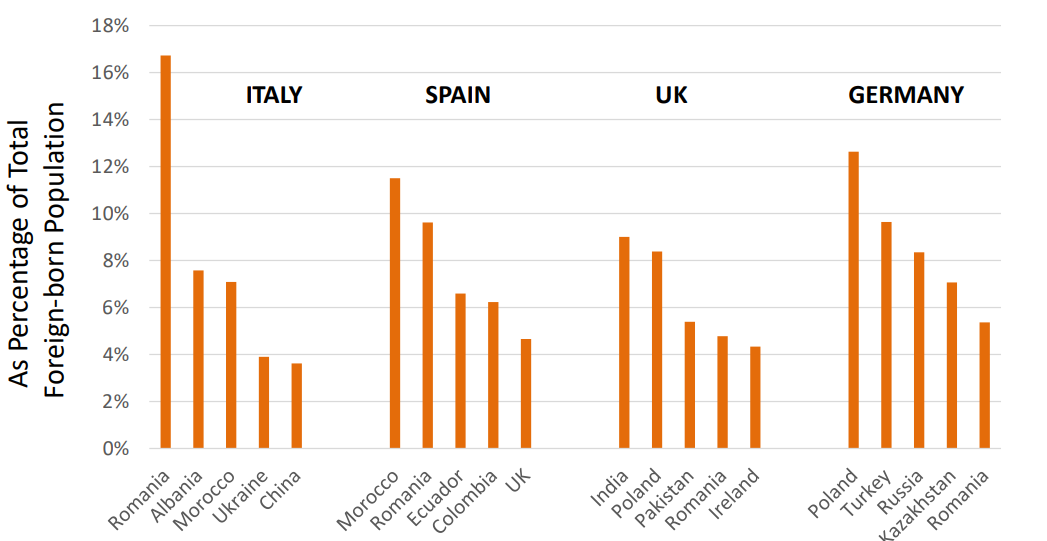
\includegraphics[width=4in]{images/ch11/5.png}
                \caption{Composition of Foreign-Born Population - Main Origin Countries, 2018}
            \end{figure}

            There is little overlap in the main origin countries of immigrants across host countries.

        \subsubsection{Employment Rate}
        
            We want to integrate and assimilate immigrants to realise their economic potential, as this is a win-win situation. When immigrants get higher wages in the host country, they pay more taxes.
            
            \begin{figure}[H]
                \centering
                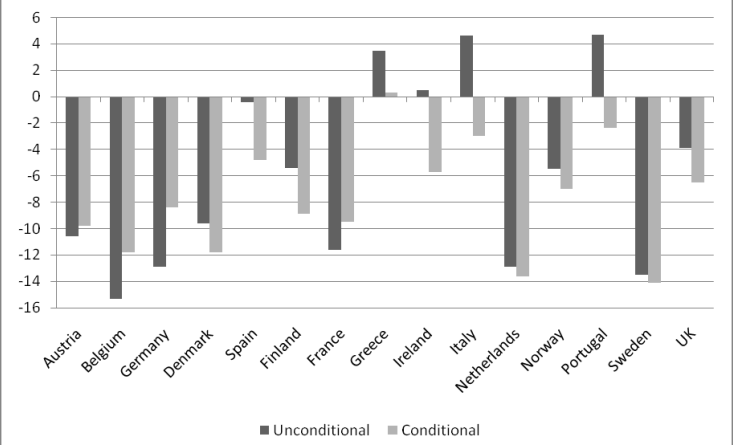
\includegraphics[width=4in]{images/ch11/7.png}
                \caption{Immigrant-native employment differential}
            \end{figure}

            Negative bars indicate that there is a higher employment probability of natives than immigrants. Positive bars indicate that there is a higher employment probability of immigrants than natives (e.g. Greece). Southern European countries tend to have positive bars unconditionally. Their shares of immigrants are small, and immigrants come only for joining the labour markets.
            
            Dark grey bars: unconditional; Light grey bars: conditional (controlling for observed characteristics such as education, labour market experience).

        \subsubsection{Position in Earnings Distribution}

            Immigrants:
            \begin{figure}[H]
                \centering
                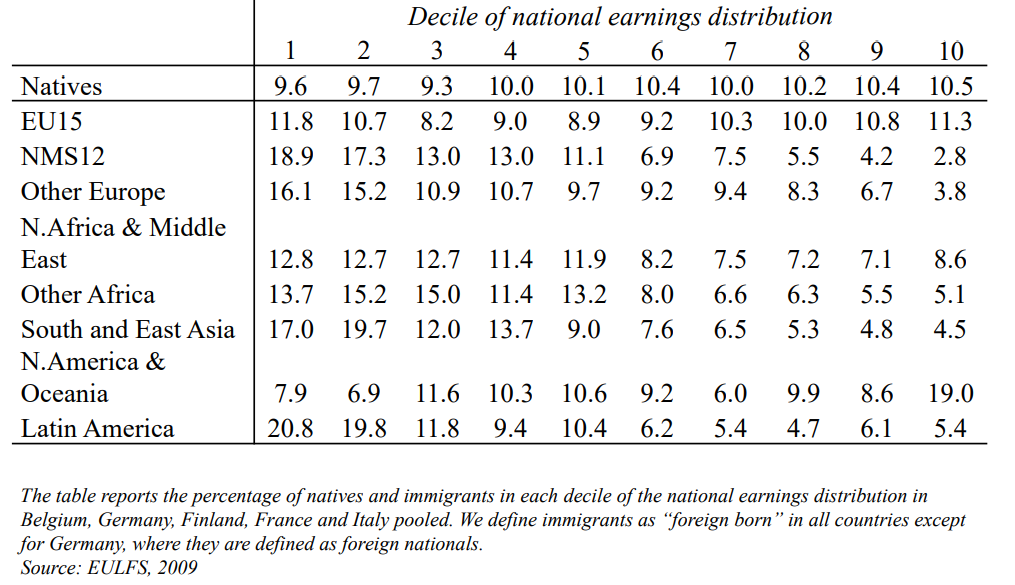
\includegraphics[width=4in]{images/ch11/8.png}
                \caption{Positions in National Earnings Distribution}
            \end{figure}
            \begin{itemize}
                \item  The table reports \emphb{the percentage of natives and immigrants in each decile} of the national earnings distribution in Belgium, Germany, Finland, France and Italy pooled. We define immigrants as “foreign born” in all countries except for Germany, where they are defined as foreign nationals.
                \item EU15 and Oceania have a relatively larger share of immigrants in the top 10 percent decile of the earnings distribution, while other continents have relatively more immigrants in the lowest 10 percent decile. 
                \item Let's show the idea of this table in a graph below (only looking at EU and non-EU immigrants).
            \end{itemize}

            Immigrants and Natives:
            
            \begin{figure}[H]
                \centering
                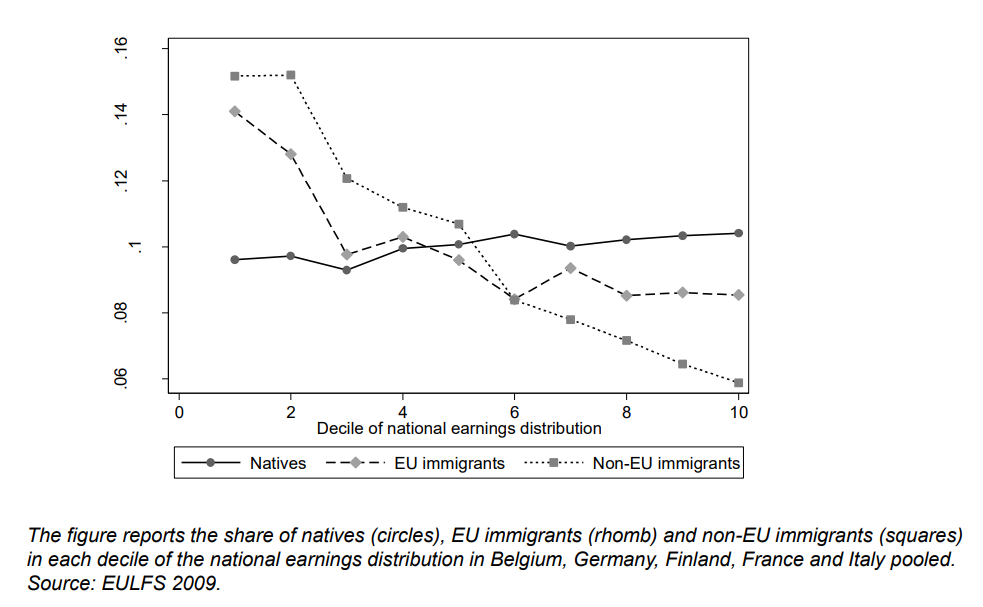
\includegraphics[width=5in]{images/ch11/9.png}
                \caption{Immigrant and native earnings distribution}
            \end{figure}
            
            \begin{itemize}
                \item The figure reports \emphb{the share of natives (circles), EU immigrants (rhomb) and non-EU immigrants (squares) in each decile} of the national earnings distribution in Belgium, Germany, Finland, France and Italy pooled.
                \item We can see the natives' line is nearly a straight line. However,  EU immigrants and non-EU immigrants have a larger proportion in the lowest 10 percent decile of the earnings distribution (e.g. 15 percent of non-EU immigrants is in this decile), and they have a smaller proportion in the top 10 percent decile (e.g. only 6 percent of non-EU immigrants is in this decile). 
            \end{itemize}

        \subsubsection{Children of Immigrants}

            \begin{figure}[H]
                \centering
                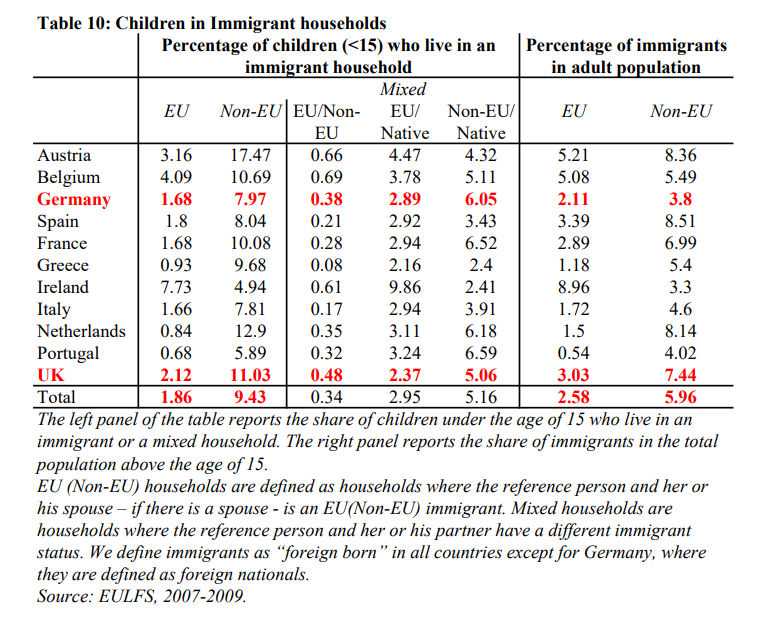
\includegraphics[width=4in]{images/ch11/10.png}
                \caption{Children of Immigrants}
            \end{figure}
            
            \begin{itemize}
                \item The left panel of the table reports \emphb{the share of children under the age of 15 who live in an immigrant or a mixed household}. The right panel reports \emphb{the share of immigrants in the total population above the age of 15}.
            \end{itemize}

        \subsubsection{Poverty}

            \begin{figure}[H]
                \centering
                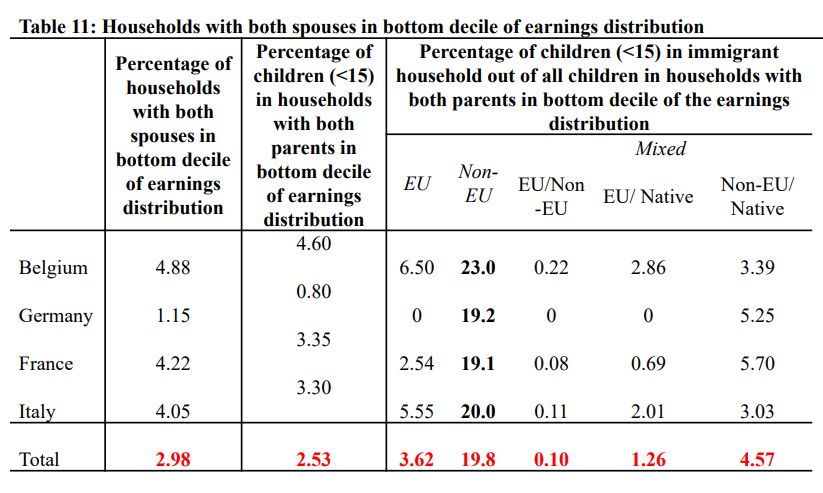
\includegraphics[width=4in]{images/ch11/11.png}
                \caption{Households with both spouses in the bottom decile of earnings distribution}
            \end{figure}
            \begin{itemize}
                \item The left panel shows the percentage of households with both spouses in the bottom decile of earnings distribution. The middle panel shows the percentage of children ($<$15) in households with both parents in the bottom decile of earnings distribution, which is quite in line with the left panel. The right panel shows \emphb{the percentage of children ($<$15) in immigrant households out of all children in households with both parents in the bottom decile of the earnings distribution}.      
                \item One in five (around 20 percent) of children ($<$15) in non-EU immigrant households live in poverty.
            \end{itemize}
            

\section{$\star$ The Migration Decision}

    \subsection{2 Main Reasons for Migration \& Refugee Protections}

        \subsubsection{2 Reasons for Migration}

            Two main reasons for migrations:
            \begin{itemize}
                \item \emphb{Forced movement} due to natural disaster or persecution
                \item \emphb{Economic motivated migration} for better economic prospects in other areas
            \end{itemize}
            
            This is still a distinction we draw today: between regulations for “asylum” immigrants and “economic” immigrants (1951 Geneva Refugee Convention).
            
            “Asylum” immigrants are not allowed to work in many countries, while economic immigrants can get access to the labour market.
            
            We will only discuss economically motivated migrations here.

        \subsubsection{Refugees and Their Protection: 1951 Geneva Convention for Refugees (GCR)}

            Who is a \emphb{Refugee}? 1951 Geneva Convention for Refugees (GCR) defines as: “[a person who] owing to a well-founded fear of being persecuted for reasons of race, religion, nationality, membership of a particular social group or political opinion, is outside the country of his nationality and is unable or, owing to such fear, is unwilling to avail himself of the protection of that country;...
            
            As of April 2015, 145 states have signed the 1951 Convention and 142 have signed both the Convention and the 1967 Protocol which endows the GCR with universal coverage. 
            
            This does not address civilians fleeing wars and conflicts (covered in different forms of temporary/subsidiary humanitarian protection).

    \subsection{Classification of Migrations}

        \begin{figure}[H]
            \centering
            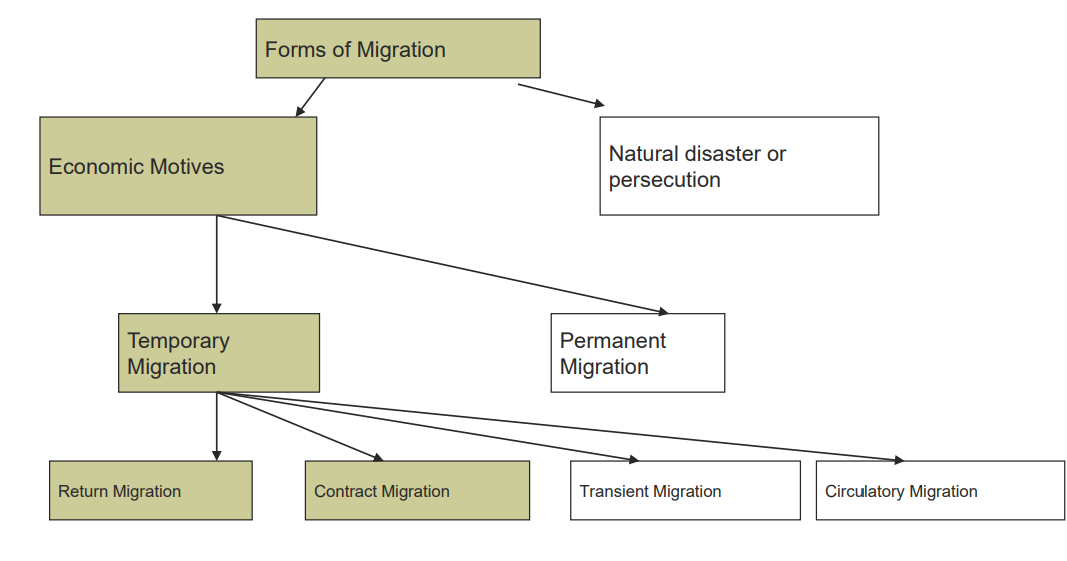
\includegraphics[width=4in]{images/ch11/12.png}
            \caption{Classification of Migrations}
        \end{figure}

    \subsection{$\star$ The Migration Decision Model}

        Migration decision of individual $i$ from $O$ to $D$ depends on the comparison of the discounted flow of future earnings in $O$ and $D$ ($y_{it}^O$ and $y_{it}^D$) net of migration cost $C_i$:
        
        \[\color{red} K_i = \sum_{t=0}^{T} y_{it}^D \frac{1}{{(1+r)}^t} - \sum_{t=0}^{T} y_{it}^O \frac{1}{{(1+r)}^t} - C_i\]

        Migration takes place whenever $K_i>0$.


\section{$\star$ Assimilation and performance of immigrants in the host countries}

    \subsection{Early Literature: \cite{chiswick_effect_1978}}

        \subsubsection{Overview}

            Large literature in the economics of migration that is concerned with the estimation of immigrants’ earnings profiles.
            
            First papers (e.g. \cite{chiswick_effect_1978}) are based on cross-section data (ignoring cohort effects) and assume migrations to be permanent (ignoring selective out-migration). Both assumptions are problematic, and we will discuss them in turn.

        \subsubsection{Empirical Strategy}

            Log wage equations, for immigrants (I) and natives (N) :

            \begin{equation*}
                \color{red}
                \begin{cases}
                    \ln w_{i}^I  & = b_{1}^IX_{i} + b_{2}^IEX_{i} + b_{3}^IYSM_{i} + e_{i}^I \\
                    \ln w_{i}^N  & = b_{1}^NX_{i} + b_{2}^NEX_{i} + e_{i}^N
                \end{cases}
            \end{equation*}

            where:
            
            \begin{itemize}
                \item $EX_i$: potential experience (computed as Age-years of schooling - 6)
                \item $YSM_i$: Years since migration
                \item $b_2^I$: measures the return to one year of total working experience (experience in host \& home country)
                \item $b_3^I$: additional increase in earnings each year spent in host country
                \item $b_2^I+b_3^I$: earnings increase per year in the host country
                \item $b_2^N$: earnings increase of natives per year of labour market experience
            \end{itemize}

            If $b_2^I+b_3^I > b_2^N$, earnings of immigrants grow faster in the host country than earnings of natives (\emphb{assimilation}).
            
            $\delta=b_2^I+b_3^I-b_2^N$ measures the \emphb{rate of convergence} of immigrant/native earnings, which represents the degree of economic assimilation.

            \begin{figure}[H]
                \centering
                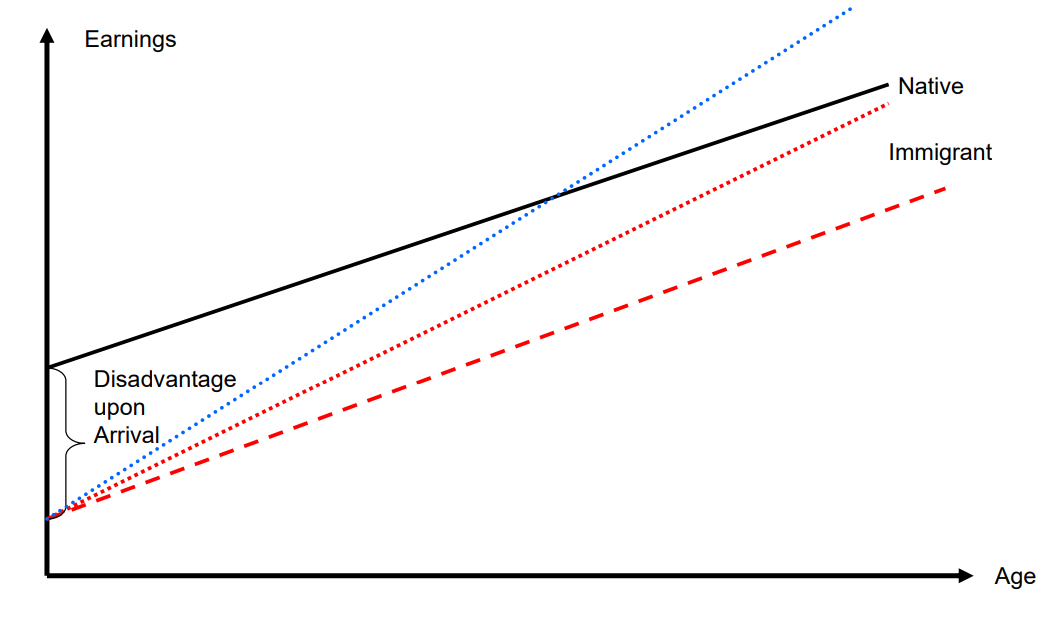
\includegraphics[width=4in]{images/ch11/13.png}
                \caption{Economic Assimilation}
            \end{figure}

        \subsubsection{Empirical Findings}

            \cite{chiswick_effect_1978} uses 1970 US census data to estimate a regression similar to the one above.
            
            Main Findings:
            
            \begin{itemize}
                \item Immigrants have upon arrival an earnings disadvantage of about 17 percent
                \item After about 10-15 years in the US labour market, earnings of immigrants overtake those of native workers.
            \end{itemize}
            
            He explains this finding with immigrants, having “more innate ability, are more highly motivated towards labour market success, or self-finance larger investments in post-school training.”

    \subsection{Cohort Effects: \cite{borjas_assimilation_1985} and Later Literatures}

        \subsubsection{Problem of Early Literatures}

            \cite{borjas_assimilation_1985} argues that estimation based on cross-sectional data may lead to misleading conclusions, because immigrants who differ in their years of residence in the host country have also arrived at different points in time. (\emphb{Cohort Effects})
            
            If entry wages of immigrants change over time, then this may be picked up by the coefficient on the years since migration variable, confounding differences in immigrant cohort quality with assimilation.
            
            \begin{figure}[H]
                \centering
                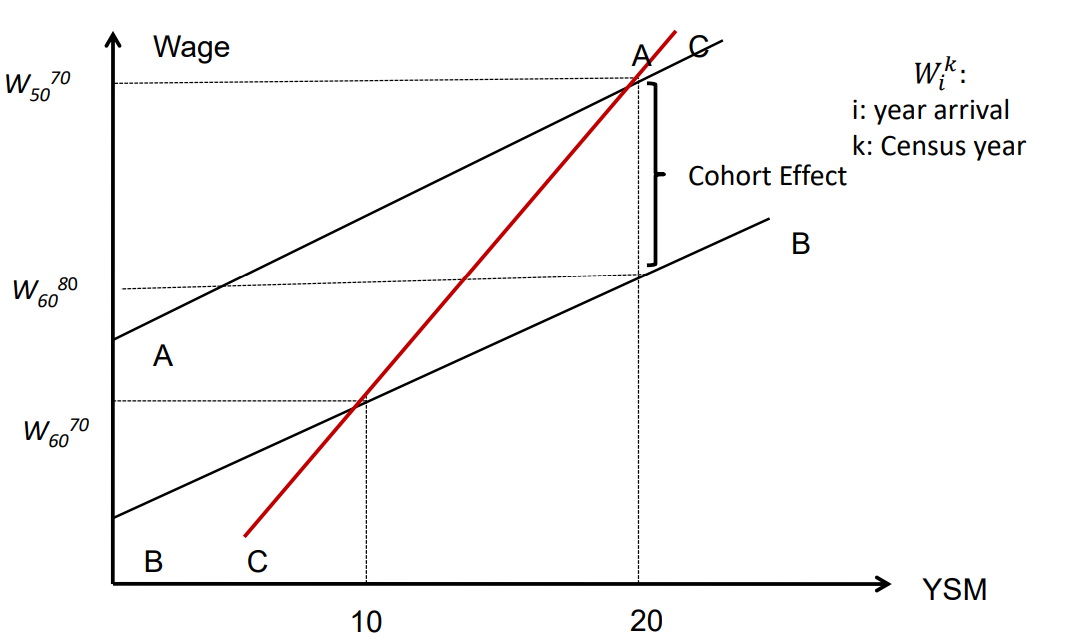
\includegraphics[width=4in]{images/ch11/14.png}
                \caption{Immigration and Assimilation: Cohort Effects}
            \end{figure}

            Formally, with 1970 census, we can observe wages for those with 20 years of residence ($w_{50}^{70}$) and for those with 10 years of residence ($w_{60}^{70}$).
            
            Estimated wage growth in host country will be:
            
            \[\color{red} \frac{\Delta w}{\Delta YSM} = \frac{w_{50}^{70}-w_{60}^{70}}{10}\]
            
            This is slope of line CC, which \empha{overestimates of immigrant wage growth if cohort effect is negative (later cohorts are worse)}. In other words, lower initial wages of subsequent cohorts may lead to an overestimate of cross-sectional wage profiles, while improvement in cohort quality leads to an underestimate.

        \subsubsection{Problem of Chiswick (Algebraically) + Deal with Cohort Effects}

            We can solve this identification problem by \empha{adding another wave of cross-section}. Suppose now we also have access to 1980 census data. We can decompose the raw wage growth:

            \begin{equation*}
                \color{red}
                \frac{w_{50}^{70} - w_{60}^{70}}{10} = \underbrace{\frac{w_{60}^{80} - w_{60}^{70}}{10}}_{\text{Wage Growth for the 1960 Cohort}} - \underbrace{\frac{w_{50}^{70} - w_{60}^{80}}{10}}_{\text{Cohort Effect}}
            \end{equation*}

            Again, we can see that:

            $$\begin{cases}
                \text{Quality improves over time} & \implies \text{Cohor Effect}<0\implies \text{Underestimatin of convergence} \\
                \text{Quality worsens over time} & \implies \text{Cohor Effect}>0\implies \text{Overestimation of convergence}
            \end{cases}$$

            To deal with this, since we have 2 cross-sections (1970, 1980) now, we can estimate:

            $$
            \Delta w=\frac{w_{50}^{70}-w_{50}^{80}}{30-20}
            $$

            However, this FD estimator can only eliminate time-unvarying fixed effect (cohort effect), but it cannot control for differences in macroeconomic conditions (time effects) in 1970 and 1980

        
        \subsubsection{Deal with Cohort Effects + Time Effects}

            To discuss this, we need to extend our estimation equations:

            \[
            \begin{cases}
            \ln w_{it}^I & = b_{1}^IX_{it} + b_{2}^IEX_{it} + b_{3}^IYSM_{it} + b_{m}^IC_{im} + \gamma_{it}^IT_{it} + e_{it}^I \\
            \ln w_{it}^N & = b_{1}^NX_{it} + b_{2}^NEX_{it} + \gamma_{t}^NT_{it} + e_{it}
            \end{cases}
            \]

            where:

            \begin{itemize}
                \item $t$ is an index indicating the year in which individual $i$ is observed
                \item $X_{it}$ is a vector of individual characteristics, e.g. gender, marital status and educational level
                \item $EX_{it}$ is potential work experience extrapolated from data
                \item $T_{it}=\mathds{1}[\text{Year of observation}=t]$ is a cross-section time indicating dummy which equals to 1 if individual $i$ is drawn from the cross-section in year $t$
                \item $\gamma_{t}^I,\gamma_{t}^N$ measure the period/time effects on log wages of immigrants and natives
                \item $C_{im}$ is an indicator function, which equals to the calendar year $m$ in which immigrant $i$ arrived
            \end{itemize}

            Problem: \empha{macro/time effect and cohort effect cannot be separately identified with repeated cross-sections $\implies$ we cannot estimate return to YSM without further assumptions.}

            Potential Solutions:

            \begin{itemize}
                \item Solution 1: \emphb{Same Cohort Effect within Group}
                    \begin{itemize}
                        \item Fix $\gamma_{t}^I$ to be the same for immigrants who arrived over a number of years (e.g. a decade)
                        \item In the extreme case where there is no time nor cohort effect, this brings us back to \cite{chiswick_effect_1978}
                        \item Assumptions like this need to be carefully justified by data: if one has strong reason to believe that the inflow of immigrants over a particular period is of roughly the same quality (for instance because immigrants all arrived from one particular source country) then this may be a plausible assumption
                    \end{itemize}
                \item Solution 2: \emphb{Same Time Effect for Immigrants and Natives}
                    \begin{itemize}
                        \item Borjas (1985) assumes that the macro/time effect is the same for immigrants and natives: $\gamma_{t}^I=\gamma_{t}^N$
                        \item Then, we can first estimate the time/macro $\gamma_{t}^N$ effects using data of natives, and use this to identify cohort effects in the immigrant equation
                        \item Nevertheless, there are evidences suggesting that change in macroeconomic conditions is likely to have different effects on wages of natives and immigrants (Dustmann, Glitz and Vogel, EER 2010)
                    \end{itemize}
                \item Solution 2+: \emphb{Parameterising Macro/Time Effects}
                    \begin{itemize}
                        \item Bratsberg et al. (2005) show that the common macro/time effect assumption leads to serious bias in assimilation profiles for the US
                        \item The provide an alternative method of estimating $\gamma$ by parameterising the macro/time effect at regional level, allowing for different variations for immigrants and natives depending on local unemployment rates
                    \end{itemize}
            \end{itemize}

    \subsection{Selective Out-migration}

        \subsubsection{Out-migration is Relevant}

            We have not yet considered \emphb{return migrations} which is indeed empirically relevant:

            \begin{figure}[H]
                \centering
                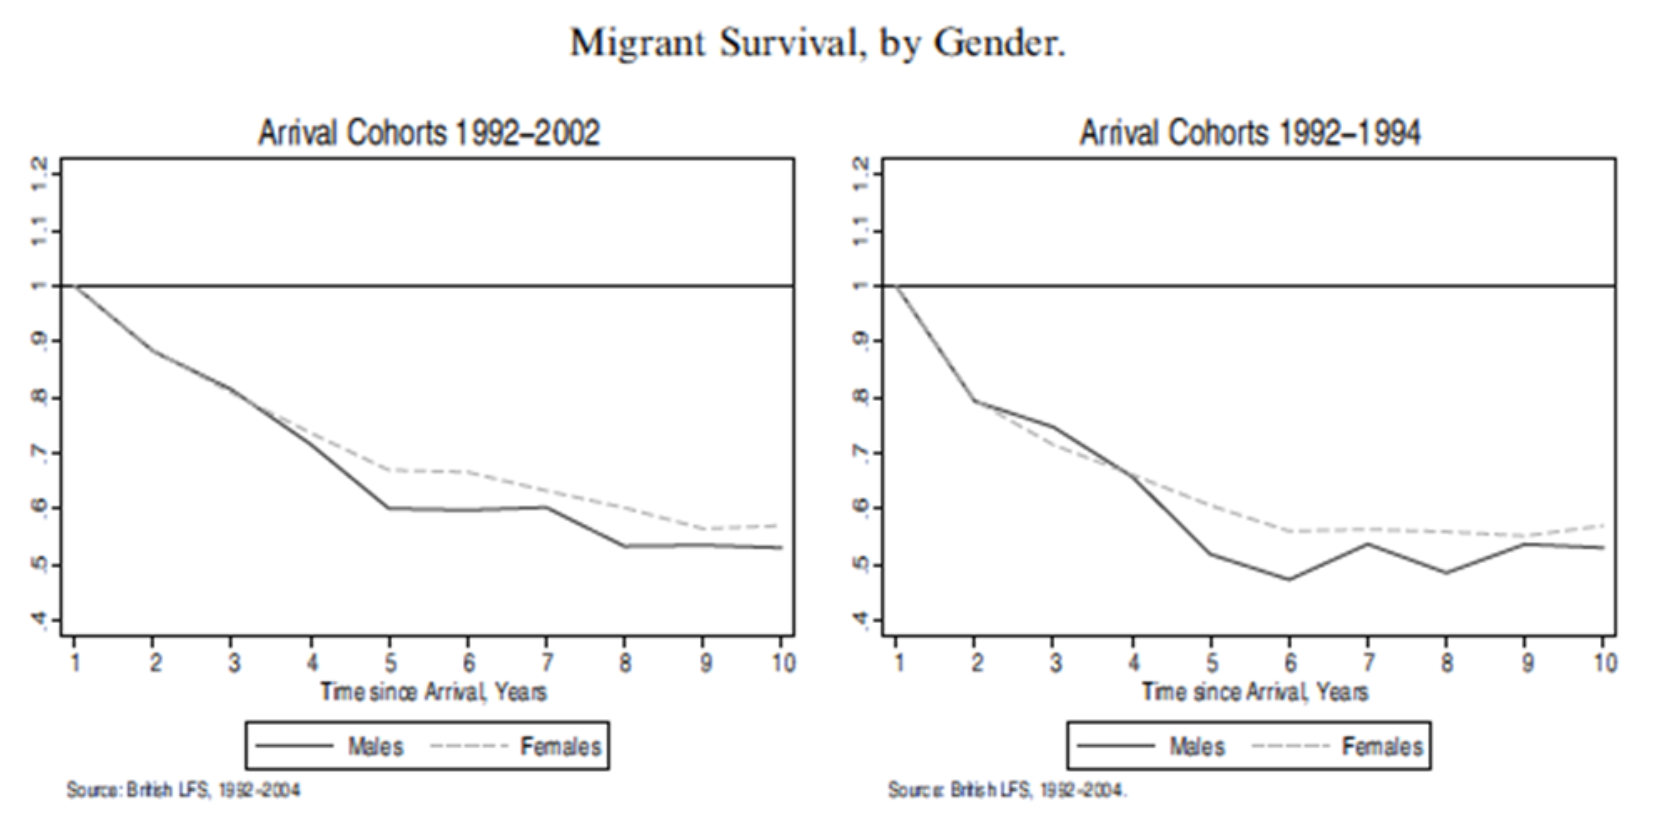
\includegraphics[width=4in]{images/ch11/11_selective_outmig_2.png}
                \caption{Immigrant Survival Rates (Dustmann and Weiss, 2007)}
            \end{figure}

            And out-migration is heterogeneous:

            \begin{figure}[H]
                \centering
                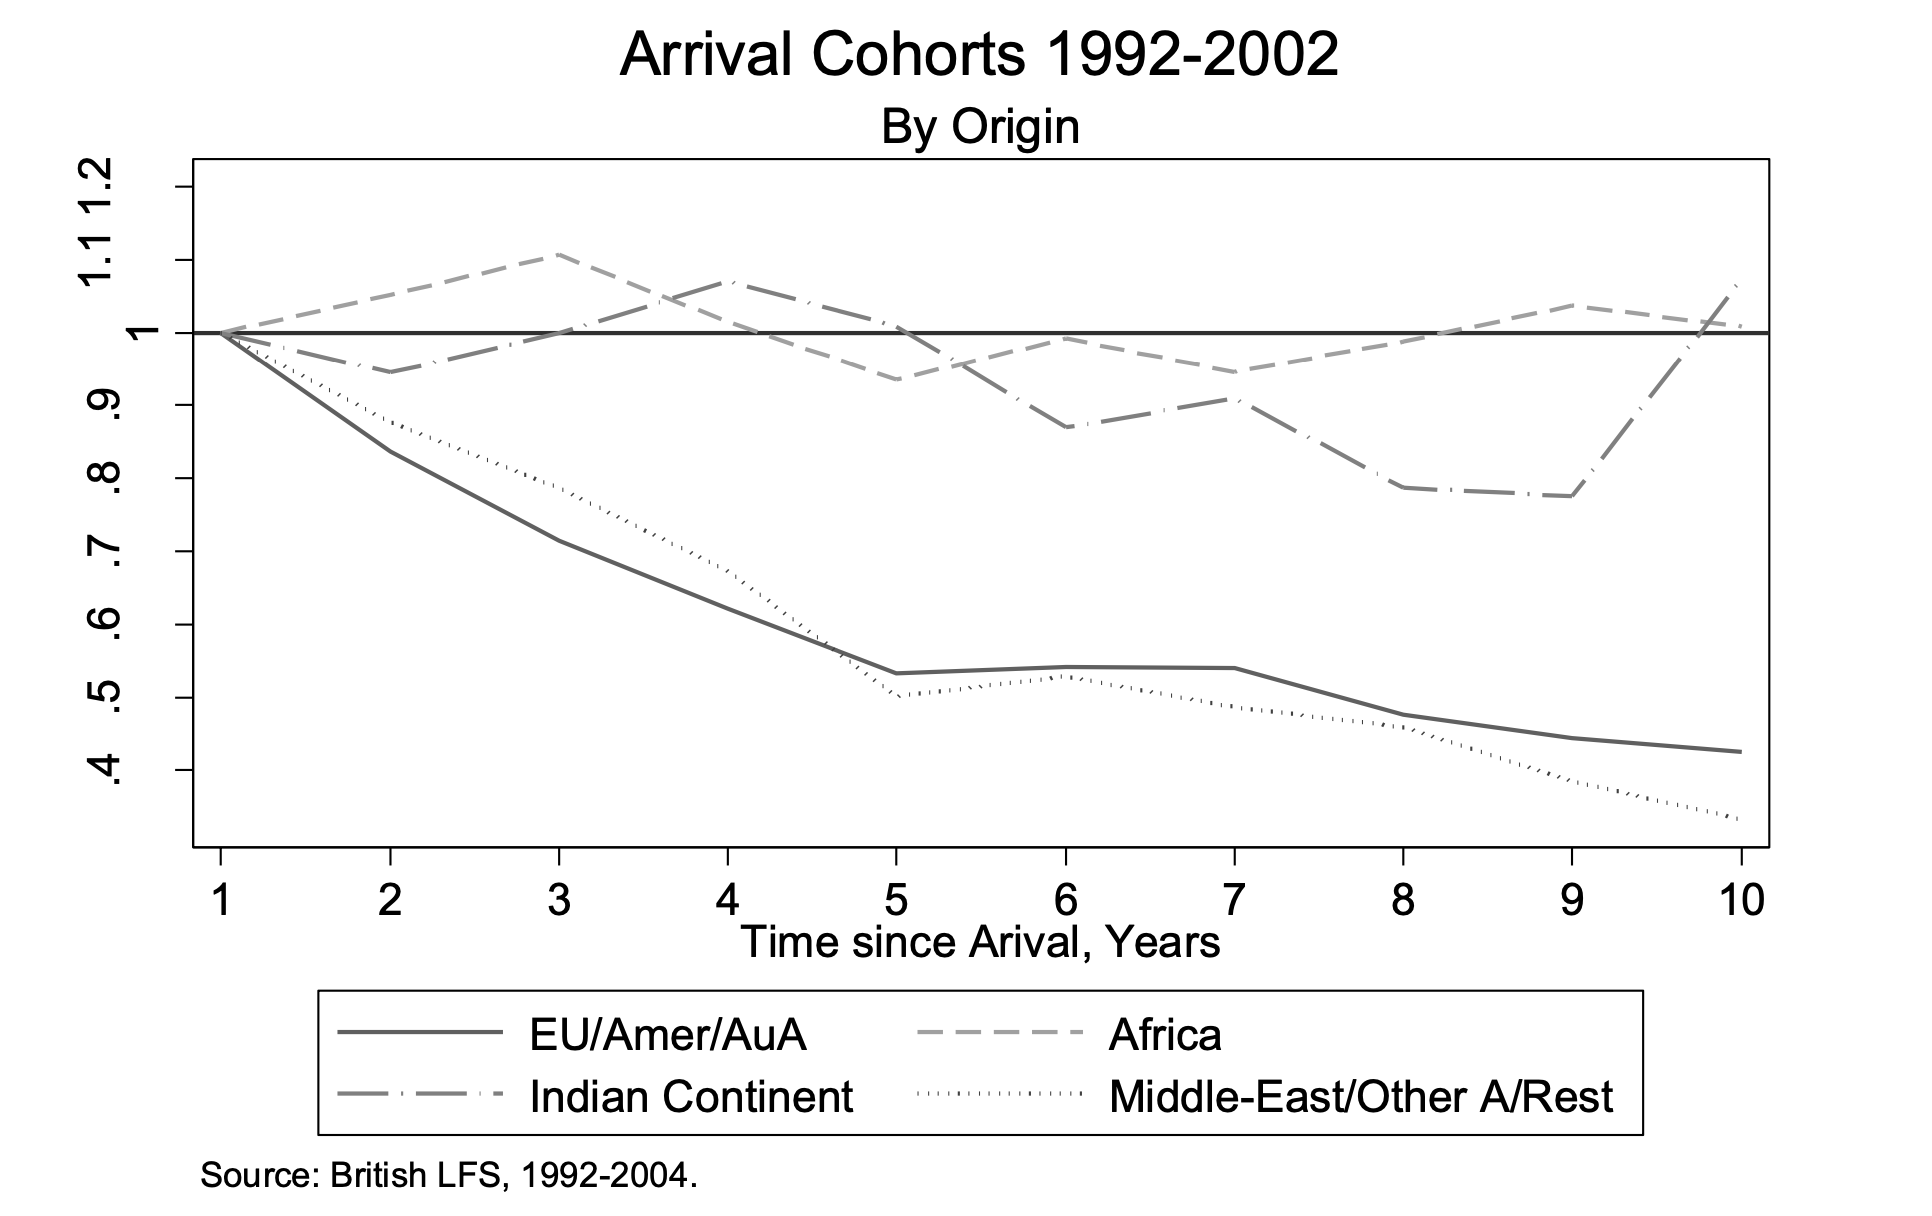
\includegraphics[width=4in]{images/ch11/11_selective_outmig_3.png}
                \caption{Immigrant Survival Rates (Dustmann and Weiss, 2007)}
            \end{figure}

        \subsubsection{Out-migration Causes Problems}

            Return migrations could lead to two problems:
            
            \begin{itemize}
                \item Return migration leads to a possibly \emphb{selective out-migration}, so that earnings profile estimates are biased
                \item Return migration may lead to \emphb{heterogeneity in the earnings paths of immigrants}, due to differences in behaviour between immigrants induced by differences in their return intentions
            \end{itemize}

        \subsubsection{Selective Out-migration}

            There is evidence of selective out-migration on education, age, and earnings; and literatures report both positively and negatively out-selection on observed characteristics. This may cause problems on the estimation of immigrants' earnings profiles:

            \begin{figure}[H]
                \centering
                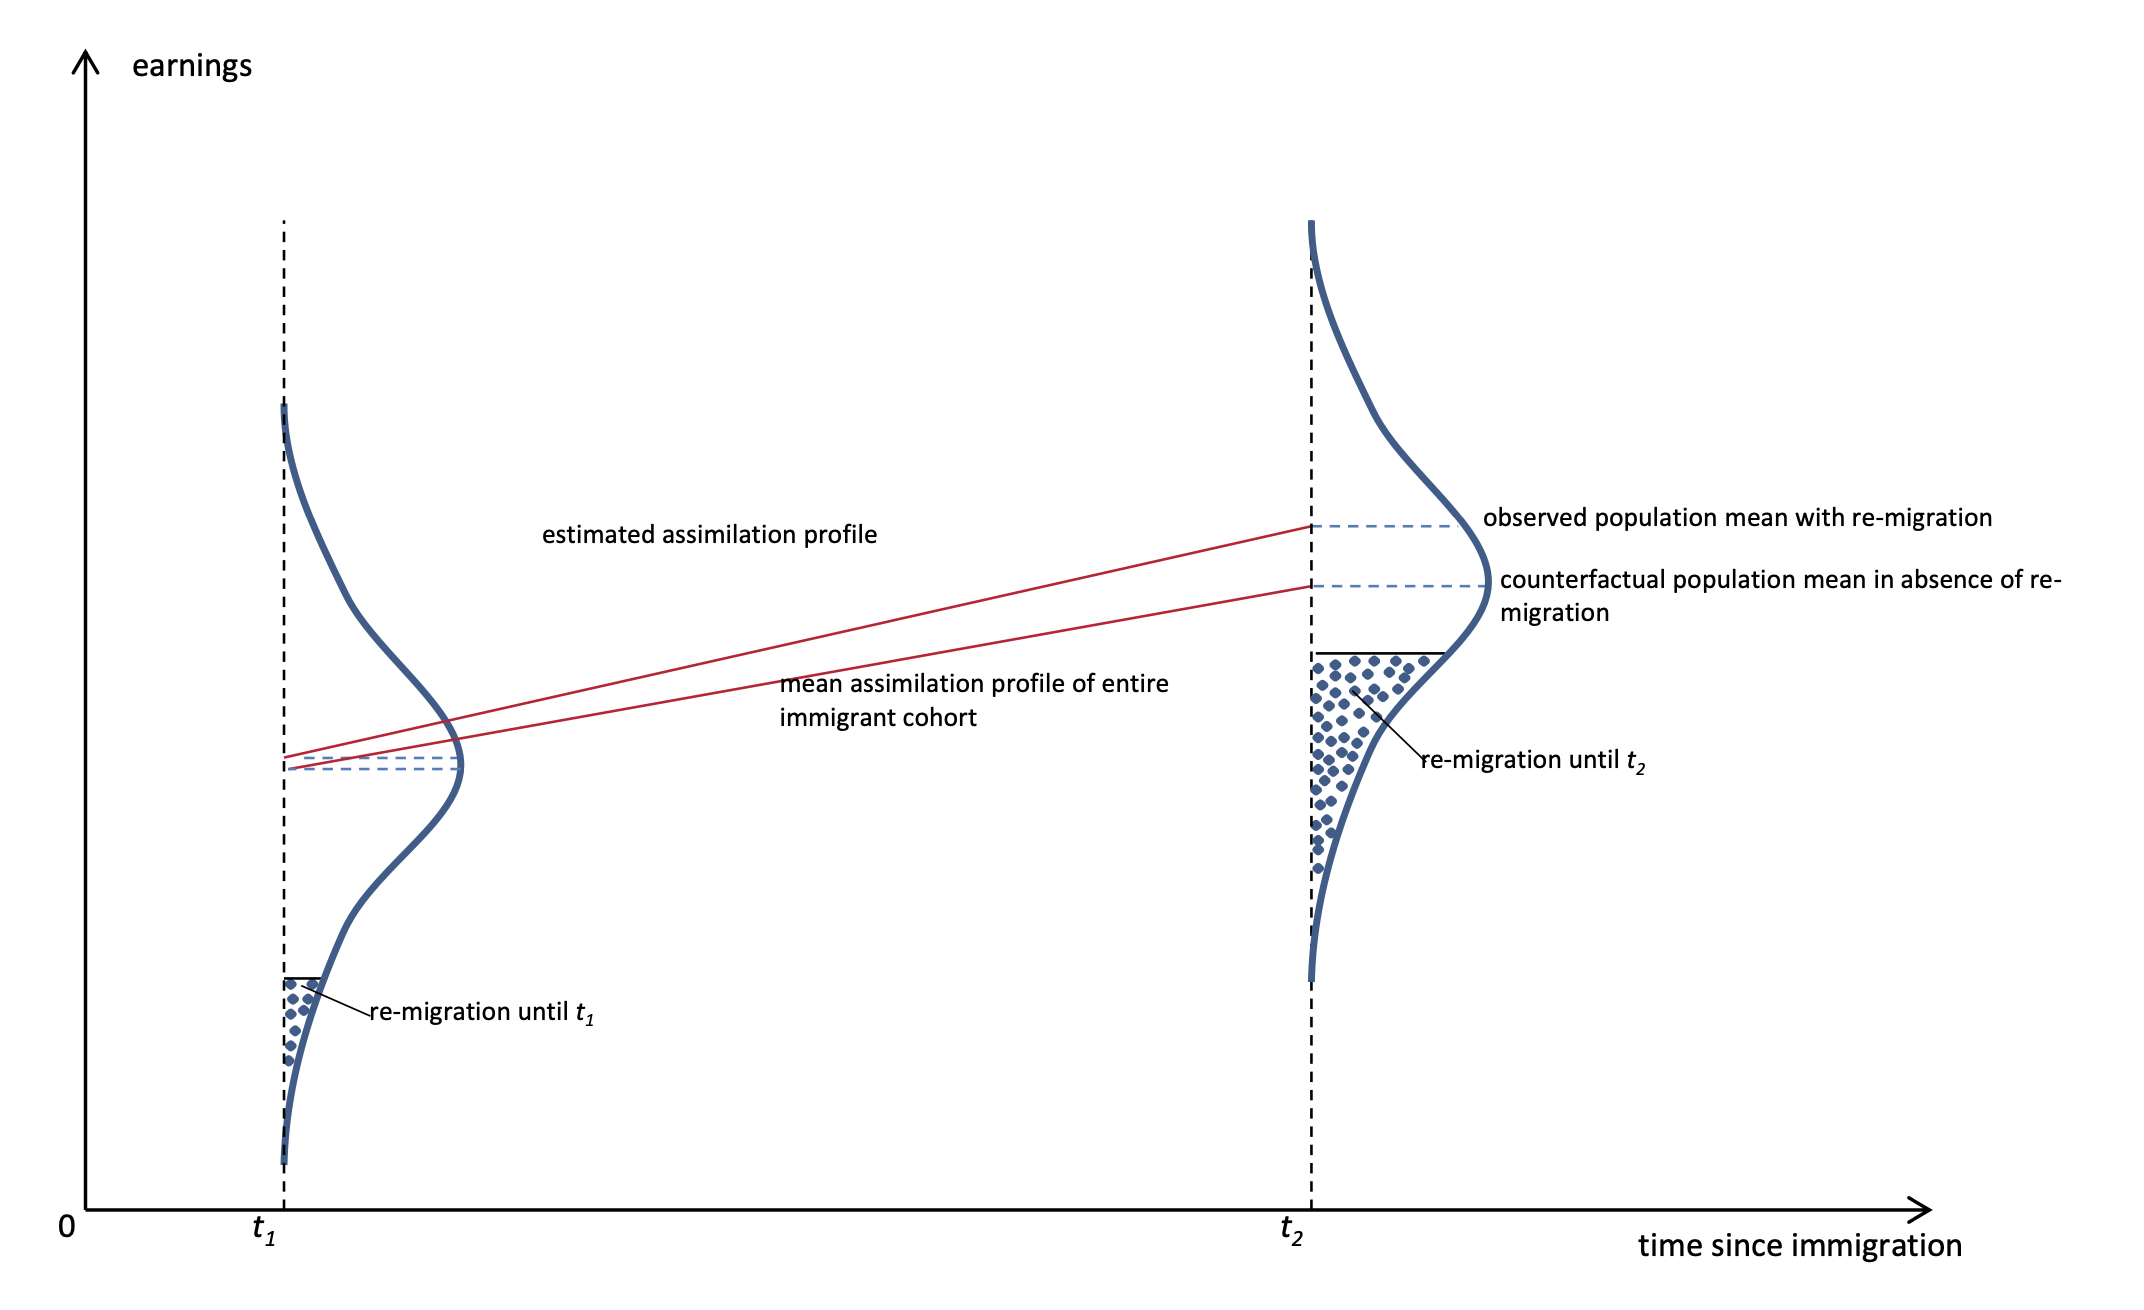
\includegraphics[width=4in]{images/ch11/11_selective_outmig_4.png}
                \caption{Assimilation Profiles, Wages (LFS, 1992-2002)}
            \end{figure}

            Ideally, we want to retrieve the lower red line while we will get the higher red line with selections. Panel data will be very useful in tackling with this issue.
    
            An example for this:
    
            \begin{figure}[H]
                \centering
                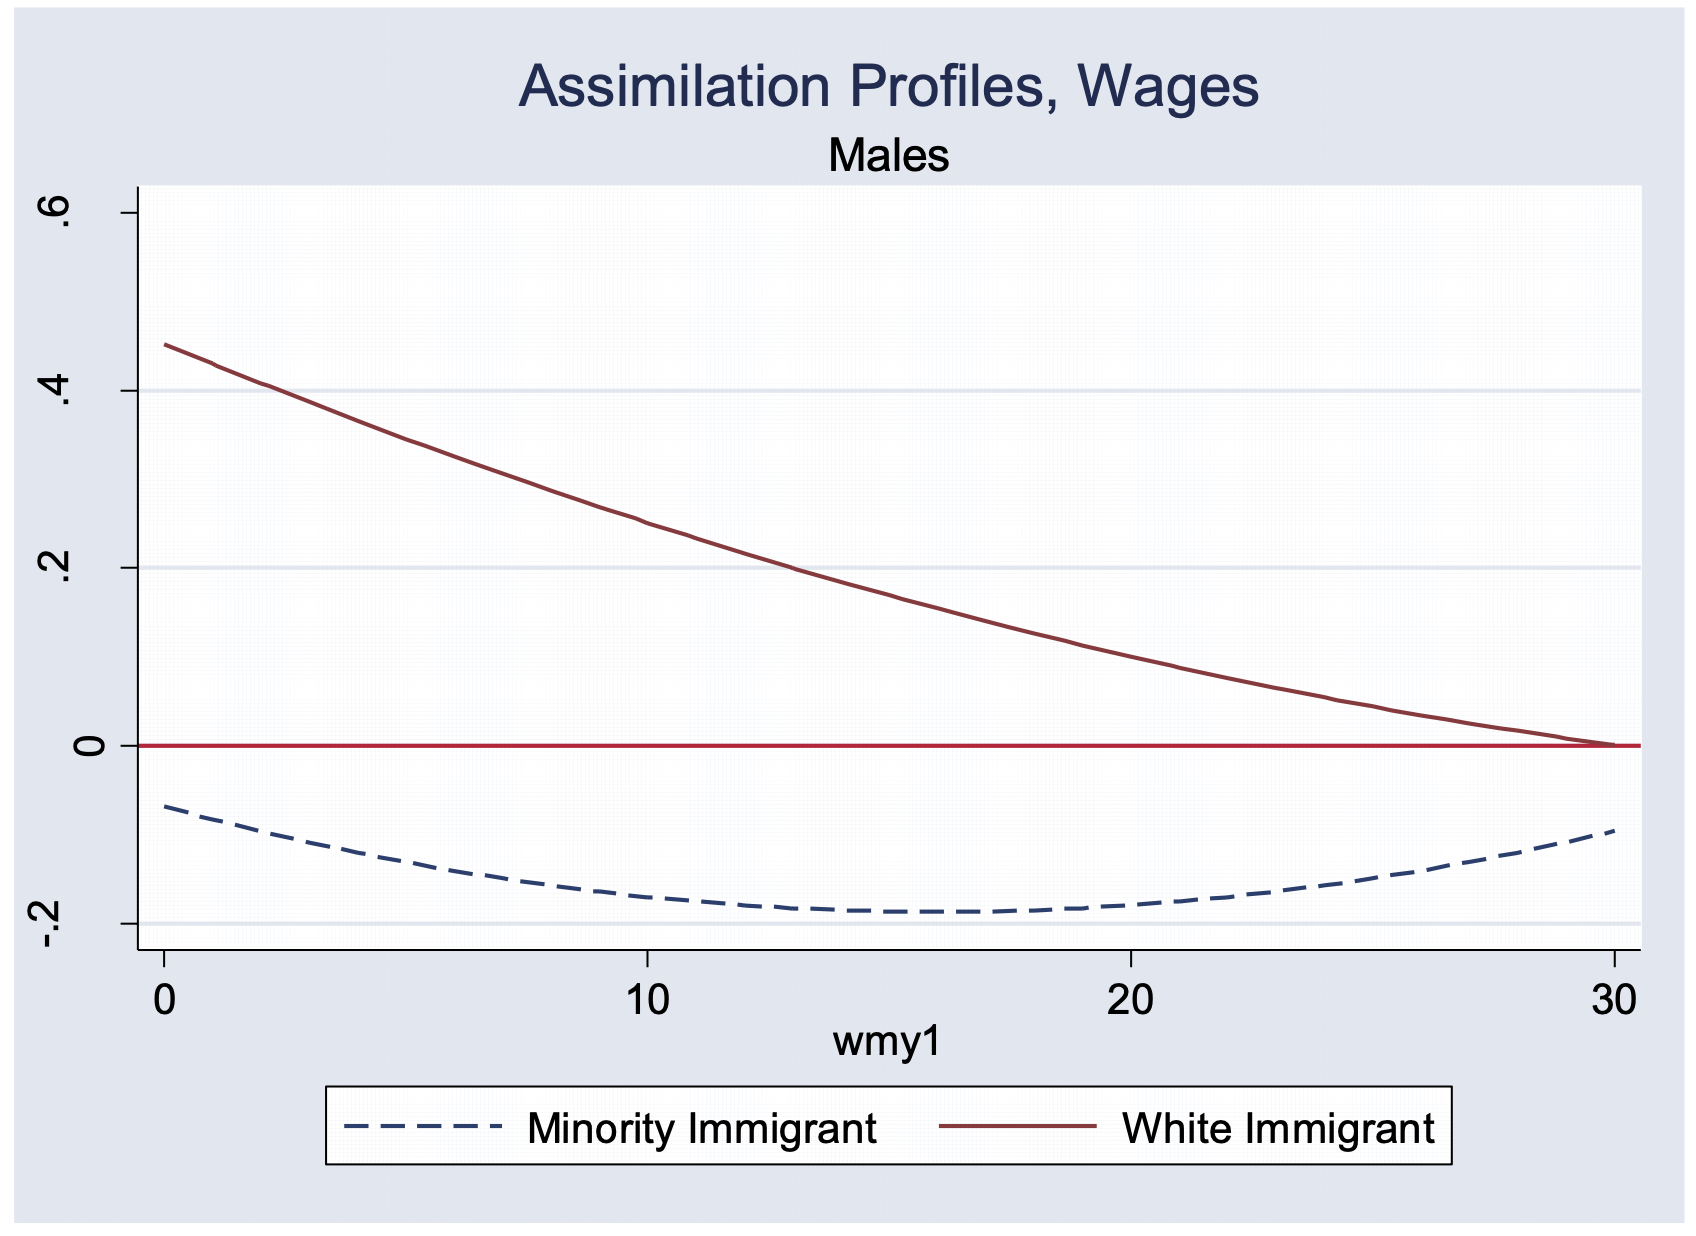
\includegraphics[width=4.5in]{images/ch11/11_selective_outmig_1.png}
                \caption{Assimilation Profiles, Wages (LFS, 1992-2002)}
            \end{figure}
    
            As shown above, what seems to be "negative assimilation" of white immigrants is actually selective out-migration where those with highest earnings leave the UK (e.g. financial workers).
    
            
    
            